\documentclass[tikz,border=2pt]{standalone}
\usepackage{amsmath,amssymb}
\usepackage{tikz}
\usetikzlibrary{arrows.meta}

\begin{document}
% The circle G(x,y) = x^2 + y^2 - 1 = 0: near a point with G_y != 0 the curve is the graph of
% a function y = g(x) (upper or lower arc); at (1, 0) and (-1, 0), where G_y = 0, no such
% graph exists — the curve is vertical there.
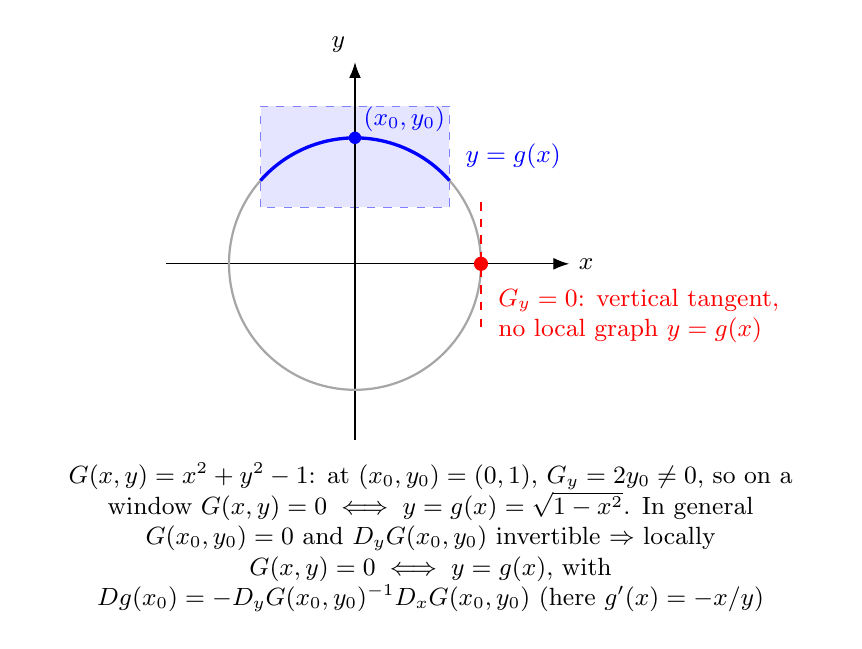
\begin{tikzpicture}[every node/.style={font=\small}, >={Latex[length=2mm]}, scale=1.6]
	\fill[blue!10] (-0.75,0.45) rectangle (0.75,1.25);
	\draw[blue!50, dashed] (-0.75,0.45) rectangle (0.75,1.25);
	\draw[->] (-1.5,0) -- (1.7,0) node[right] {$x$};
	\draw[->] (0,-1.4) -- (0,1.6) node[above left] {$y$};
	\draw[gray!70, thick] (0,0) circle (1);
	\draw[blue, very thick] (-0.75,0.661) arc (138.6:41.4:1);
	\fill[blue] (0,1) circle (1.4pt);
	\node[blue, anchor=south west, font=\small, inner sep=2pt] at (0.02,1.0) {$(x_0,y_0)$};
	\node[blue, anchor=west, font=\small] at (0.8,0.85) {$y=g(x)$};
	\fill[red] (1,0) circle (1.6pt);
	\draw[red, dashed] (1,-0.5) -- (1,0.5);
	\node[red, anchor=north west, font=\small, align=left] at (1.06,-0.12) {$G_y=0$: vertical tangent,\\ no local graph $y=g(x)$};
	\node[anchor=north, align=flush center, text width=10cm] at (0.6,-1.5) {$G(x,y)=x^2+y^2-1$: at $(x_0,y_0)=(0,1)$, $G_y=2y_0\neq0$, so on a window $G(x,y)=0\iff y=g(x)=\sqrt{1-x^2}$. In general $G(x_0,y_0)=0$ and $D_yG(x_0,y_0)$ invertible $\Rightarrow$ locally $G(x,y)=0\iff y=g(x)$, with $Dg(x_0)=-D_yG(x_0,y_0)^{-1}D_xG(x_0,y_0)$ (here $g'(x)=-x/y$)};
\end{tikzpicture}
\end{document}
